%	\section{Experiment 0: Explicit Evaluations}
%	In order to establish a baseline gender score for morphologically marked gendered occupational and social roles in English, blah...
%	
%	\subsection{Methods} 
%	
%	100 participants were recruited through the online recruitment platform `Prolific'. All participants self-identified as L1 English speakers and as having been born and in the United States, and all lived in the United States at the time of participation. None of the participants had participated in the pilot study. Finally, all participants were paid \$2.00 for their participation in the study, and spent an average of four to five minutes on the experiment (average payout \$31.86 per hour). 
%	
%	Each participant was presented with a series of sentences of the form ``Someone is a TITLE", where the title in question was one of the 39 selected titles in one of their gendered forms. Each participant saw all 39 of the lexical items in question, and 13 of each gender form (male/female/neutral), so that no participant ever saw the same lexeme in a different format (e.g. a participant would not see both \textit{congressperson} and \textit{congresswoman}). 
%	
%	Participants were asked to judge how likely it was that the `someone' in question was a man or a woman, and indicated their responses on a seven-point Likert scale. Which binary gender the left (1) or right (7) ends of the scale represented was randomized between participants but consistent within a single subject's study. For each item, participants were also permitted to check an optional box indicating that they were not familiar with the term in question, due to the relatively low frequency of some of the critical items.  Finally, all participants completed an optional post-experiment demographic survey.
%	
%	%An example of this procedure is provided in Figure \ref{norming_sample}.
%	
%%	\begin{figure*}[hb]
	%%		\centering
	%%		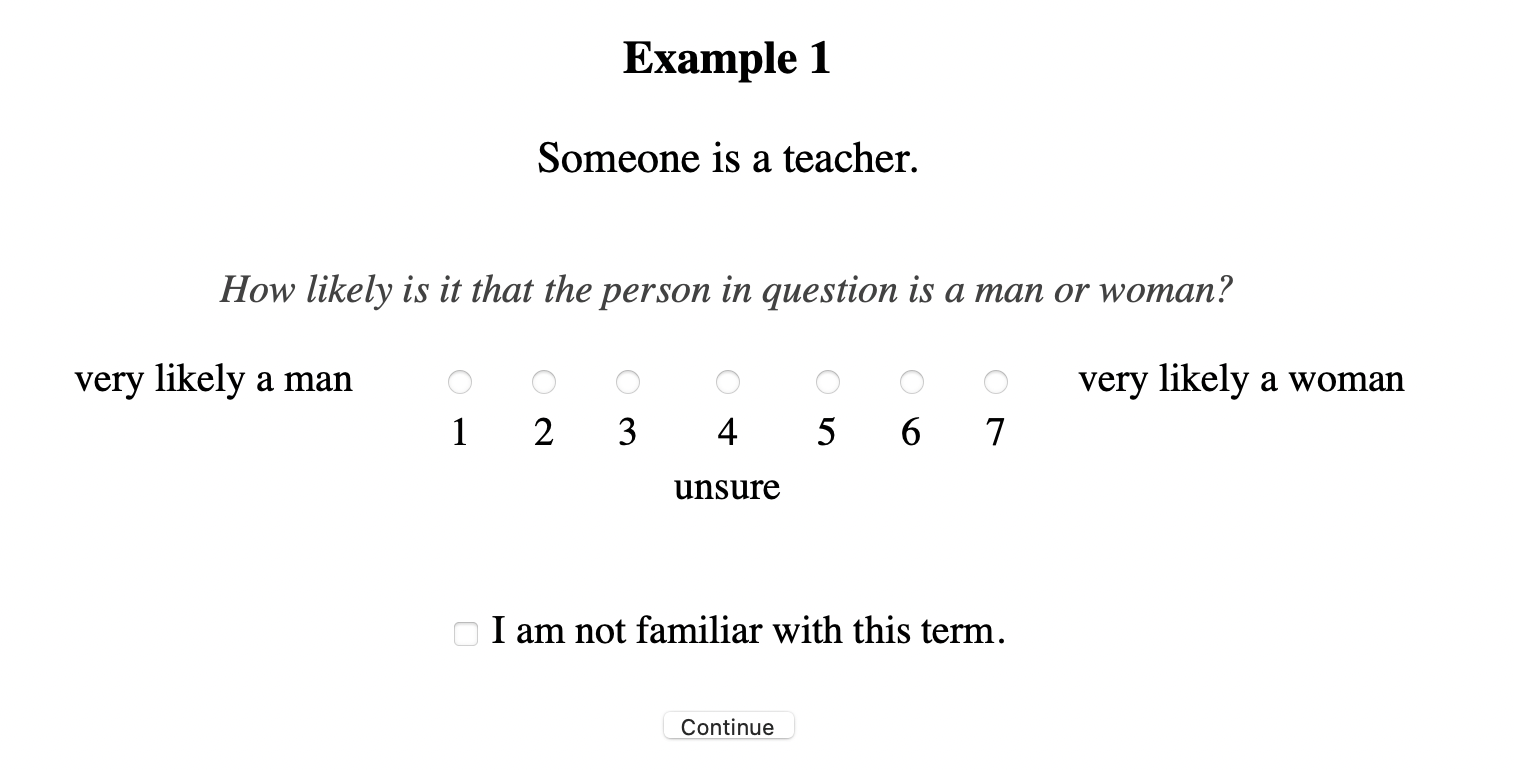
\includegraphics[scale=0.5]{norming_capture.png}
	%%		\caption{A trial of the procedure in Experiment 0, as seen by participants}
	%%		\label{norming_sample}
	%%	\end{figure*}
%	
%	
%	\subsection{Results}
%	
%	\begin{figure*}[ht]
	%		\centering
	%		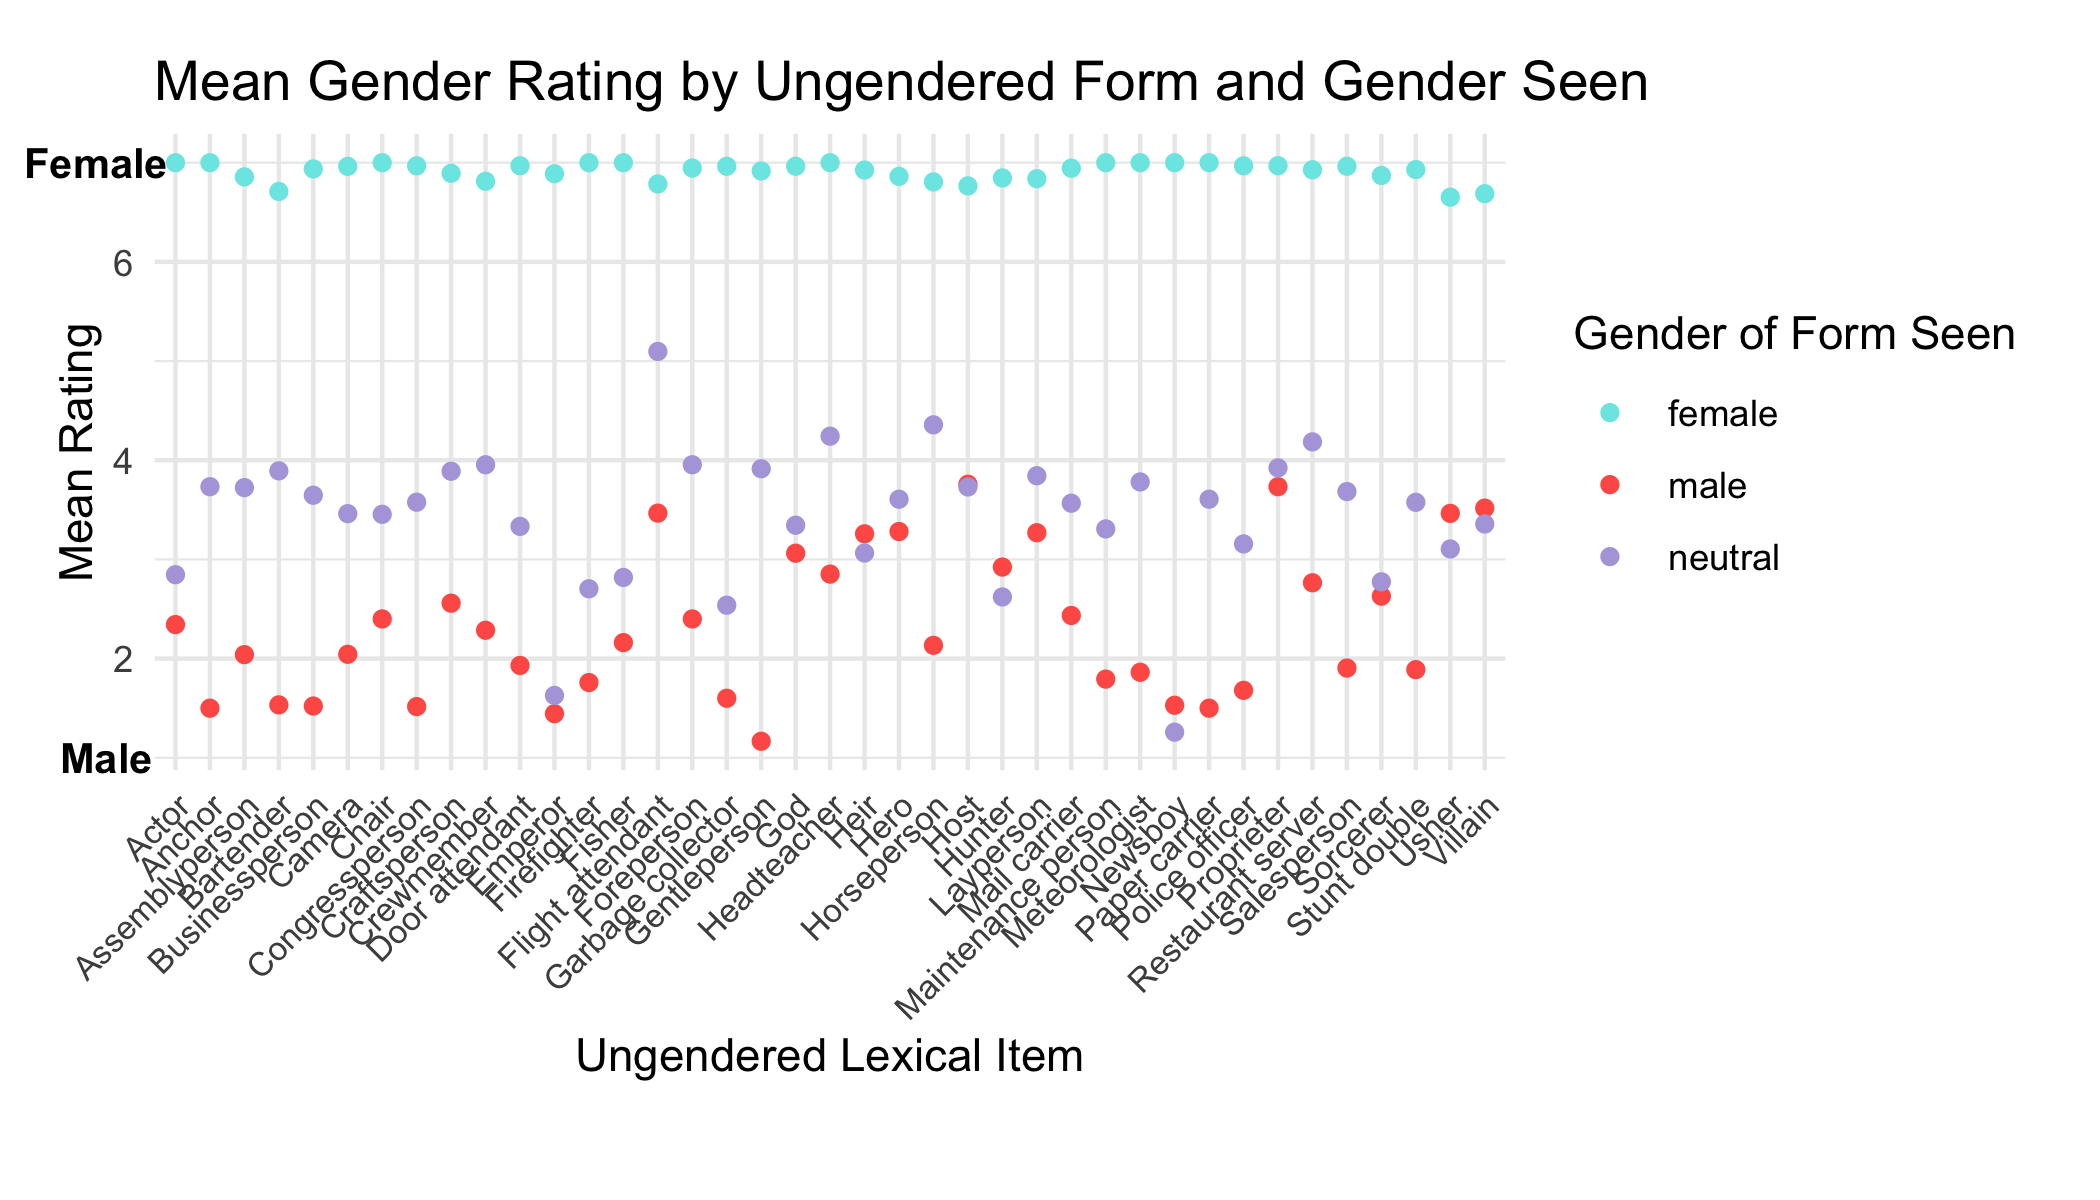
\includegraphics[scale=0.2]{norming_results_all.png}
	%		\caption{Mean gender reporting of items by lexical item and gender seen}
	%		\label{norming_results_all}
	%	\end{figure*}
\newpage
%	\section{Experiment 1: MAZE Task}
%
%	\subsection{Methods}
%	
%	\subsubsection{Participants} A total of 200 participants were collected for this task via the online recruitment platform Prolific. The task was advertised to 100 self-identifying Republicans and 100 self-identifying Democrats, in order to ensure an even distribution of political affiliations. All participants additionally self-identified as L1 English speakers and as having been born and in the United States, and all lived in the United States at the time of participation. None of the participants had participated in the pilot study or in any other study related to the present project. Finally, all participants were paid \$1.75 for their participation\footnote{With a mean completion time of 5.39 minutes, participants were paid at a rate of \$20.73/hr}. \par 
%	
%	\subsubsection{Stimuli}
%	The stimuli sentences in this experiment were of the form ``NAME is a/n TITLE from STATE. PRONOUN likes ACTIVITY"- for example, ``Brittany is a chef from Louisiana". The twenty most popular male and female names were selected from the lists of most popular names for boys and girls in 1998 according to the Social Security \citeA{socialsecurity}. Names which appeared within the top 100 entries on both lists (e.g. Taylor, Ryan) were excluded, in order to ensure that the names used in the experiment were sufficiently socially gendered. These names were randomized between participants, with no participant seeing the same name more than once. States and activities were randomized at the stimuli creation stage so that they remained constant for all participants.\par
%	The critical items in question were the forms that appeared in the TITLE location of the sentences. A total of 20 social and occupational titles which display overt morphological gender were chosen, with the majority of these showing three possible gender realizations: male, female, and neutral (e.g. \textit{congressman, congresswoman, congressperson}). The remaining items only distinguished between female and non-female forms (e.g. \textit{actress} vs. \textit{actor}). Thus, any vignette had the possibility to appear \textbf{congruent} in its gender markings (e.g. a male name with a male lexical item) or \textbf{neutral} in its congruency (e.g. a female name with a neutral lexical item)\footnote{We did not test gender-incongruent vignettes such as `David is a congresswoman', for fear that it would draw too much attention to the gendered nature of the task at hand.}. \par
%	Once the sentences were constructed, each item in the sentence was paired with a distractor item deemed to have a similar surprisal value in that same context, using the A(uto)-Maze generator developed and described in \citeA{boyce2020maze}. Where surprisal values could not be accurately obtained, for example because of low lexical frequency of the critical items, distractors were matched on orthographic length.  
%	
%	\subsubsection{Procedure}
%	The experiment consisted of an implementation of the maze task \cite{forster2009maze}, wherein participants are presented with sentences one word at a time, and each word is paired with an ungrammatical distractor. Participants are tasked with proceeding through the sentence one word at a time, selecting the grammatical continuation of the sentence by indicating a corresponding key on their keyboard, and time measures are taken of the decision time. The beginning of a sentence is always paired with an ``X-X-X", which participants are told not to select. An example of the progression of such a task is provided in Figure 1.
%	
%	\begin{figure}[ht]
	%		\centering
	%		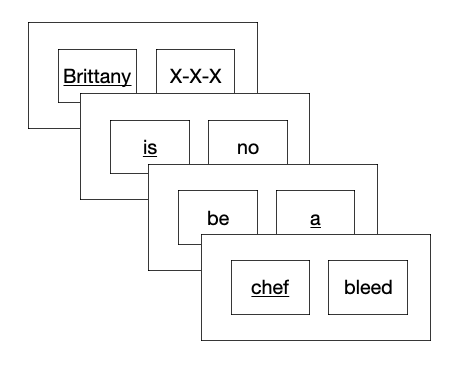
\includegraphics[scale=0.33]{maze-exe}
	%		\caption{An example of the maze task progression. Each larger frame represents a selection choice, wherein only one of the words can continue the sentence. These continuations are underlined in this example.}
	%		\label{maze-exe}
	%	\end{figure}
%	 \par 
%	If the participant successfully made it to the end of the sentence, they were asked about the state from which the character in the vignette comes. This question served both to distract participants from the question under investigation (gender) and also as an attention check. If, however, the participant failed to successfully navigate the sentence, they were prompted to continue on to the next sentence, and that item was marked as incomplete.
%
%	\subsubsection{Post-Experimental Survey}
%	In order to assess the participants' ideologies towards gender, we employ the Social Roles Questionnaire developed by \citeA{baber2006social}. This survey consists of 13 questions which are designed to elicit both implicit and explicit ideologies about gender, including the notions of gender as an immutable fact vs gender as a social construct (what Baber and Tucker term `gender transendence'), as well as about the societal roles performed by the (binary) genders (`gender linking').\par 
%	Each of the 13 questionnaire items was presented alongside a sliding scale from `strongly disagree' to `strongly agree', which corresponded to numerical values of 0 and 100, respectively. The questions related to `gender linking' were inversely coded. Participants were then assigned a gender ideology score from 0 to 100 by taking the mean of their individual responses; the closer to 0 a participant is, the more open-minded their approach to gender, and the closer to 100, the more conservative or traditional their view of gender.\par 
%	Finally, participants filled out an optional post-experimental demographic survey. This included questions about their own gender, political affiliations, and age. The full survey is available online as part of the supplementary materials.
%		
%	\subsection{Results}
%	
%	\subsubsection{Exclusions} 23 participants were excluded because they failed to meet the 80\% threshold for attention check questions. Additionally, we excluded any individual trial which deviated from the mean for that item by more than two standard deviations in order to control for the effects of outliers. This resulted in an additional 142 observations being excluded, for a total of 3271 observations left for analysis.  
%	
%	\begin{figure}[ht]
	%		\centering
	%		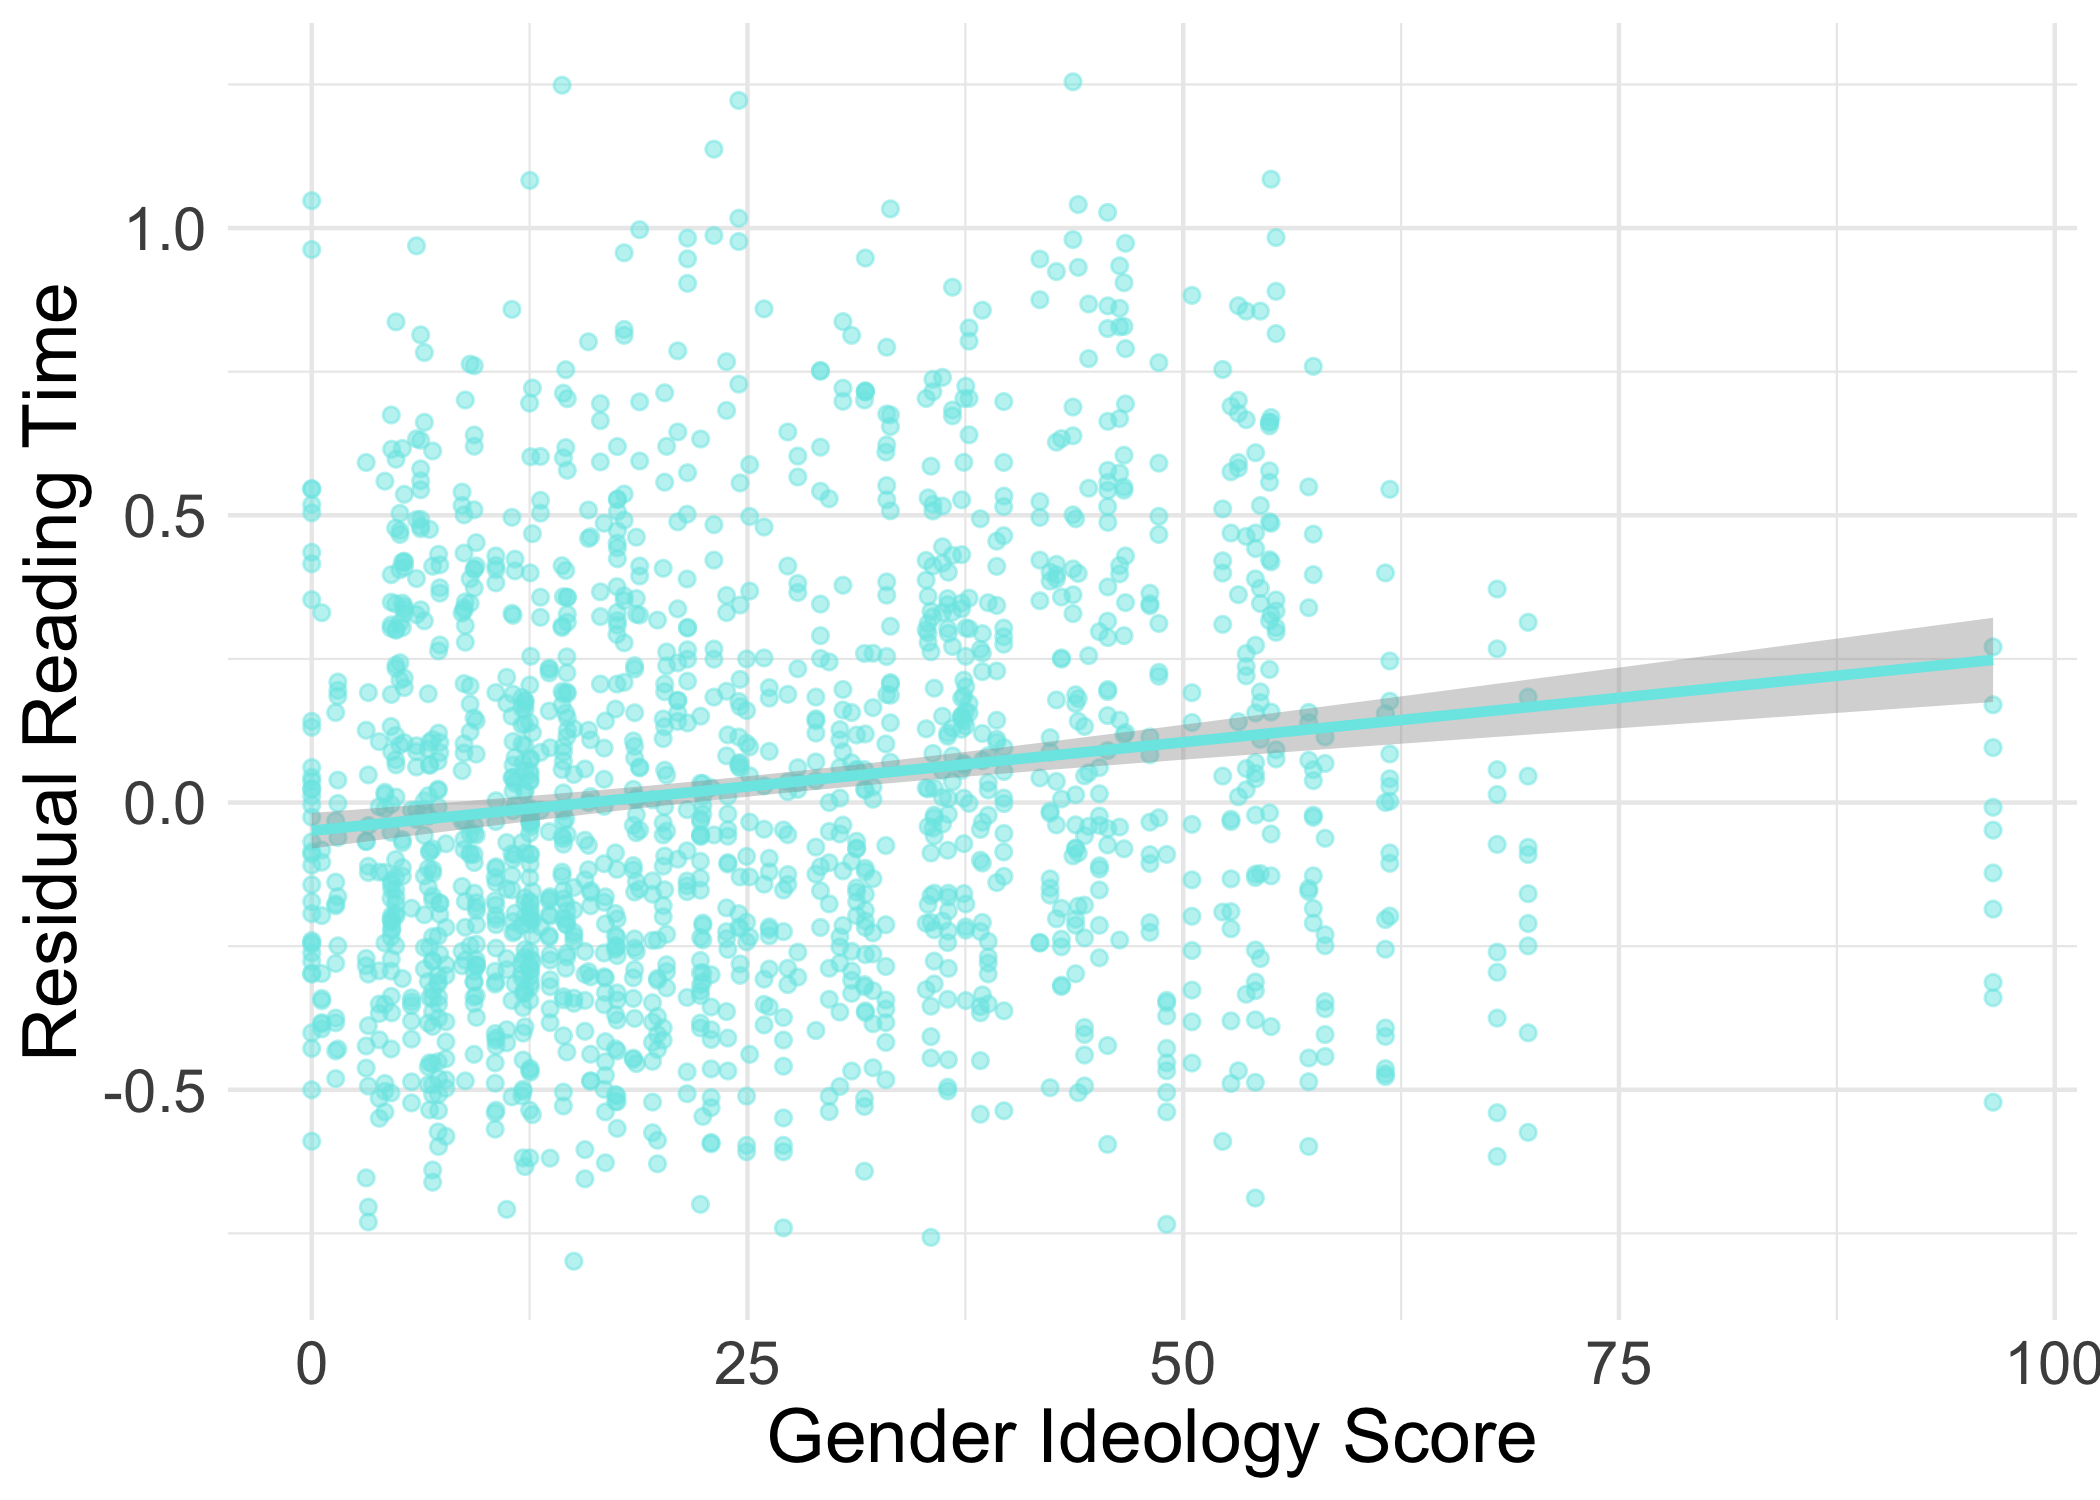
\includegraphics[scale=0.115]{maze_neutral_all.png}
	%		\caption{Average residual decision time on gender-neutral forms in Experiment 1.}
	%		\label{maze_neutral_all}
	%	\end{figure}
%	
%	\begin{figure}[ht]
	%		\centering
	%		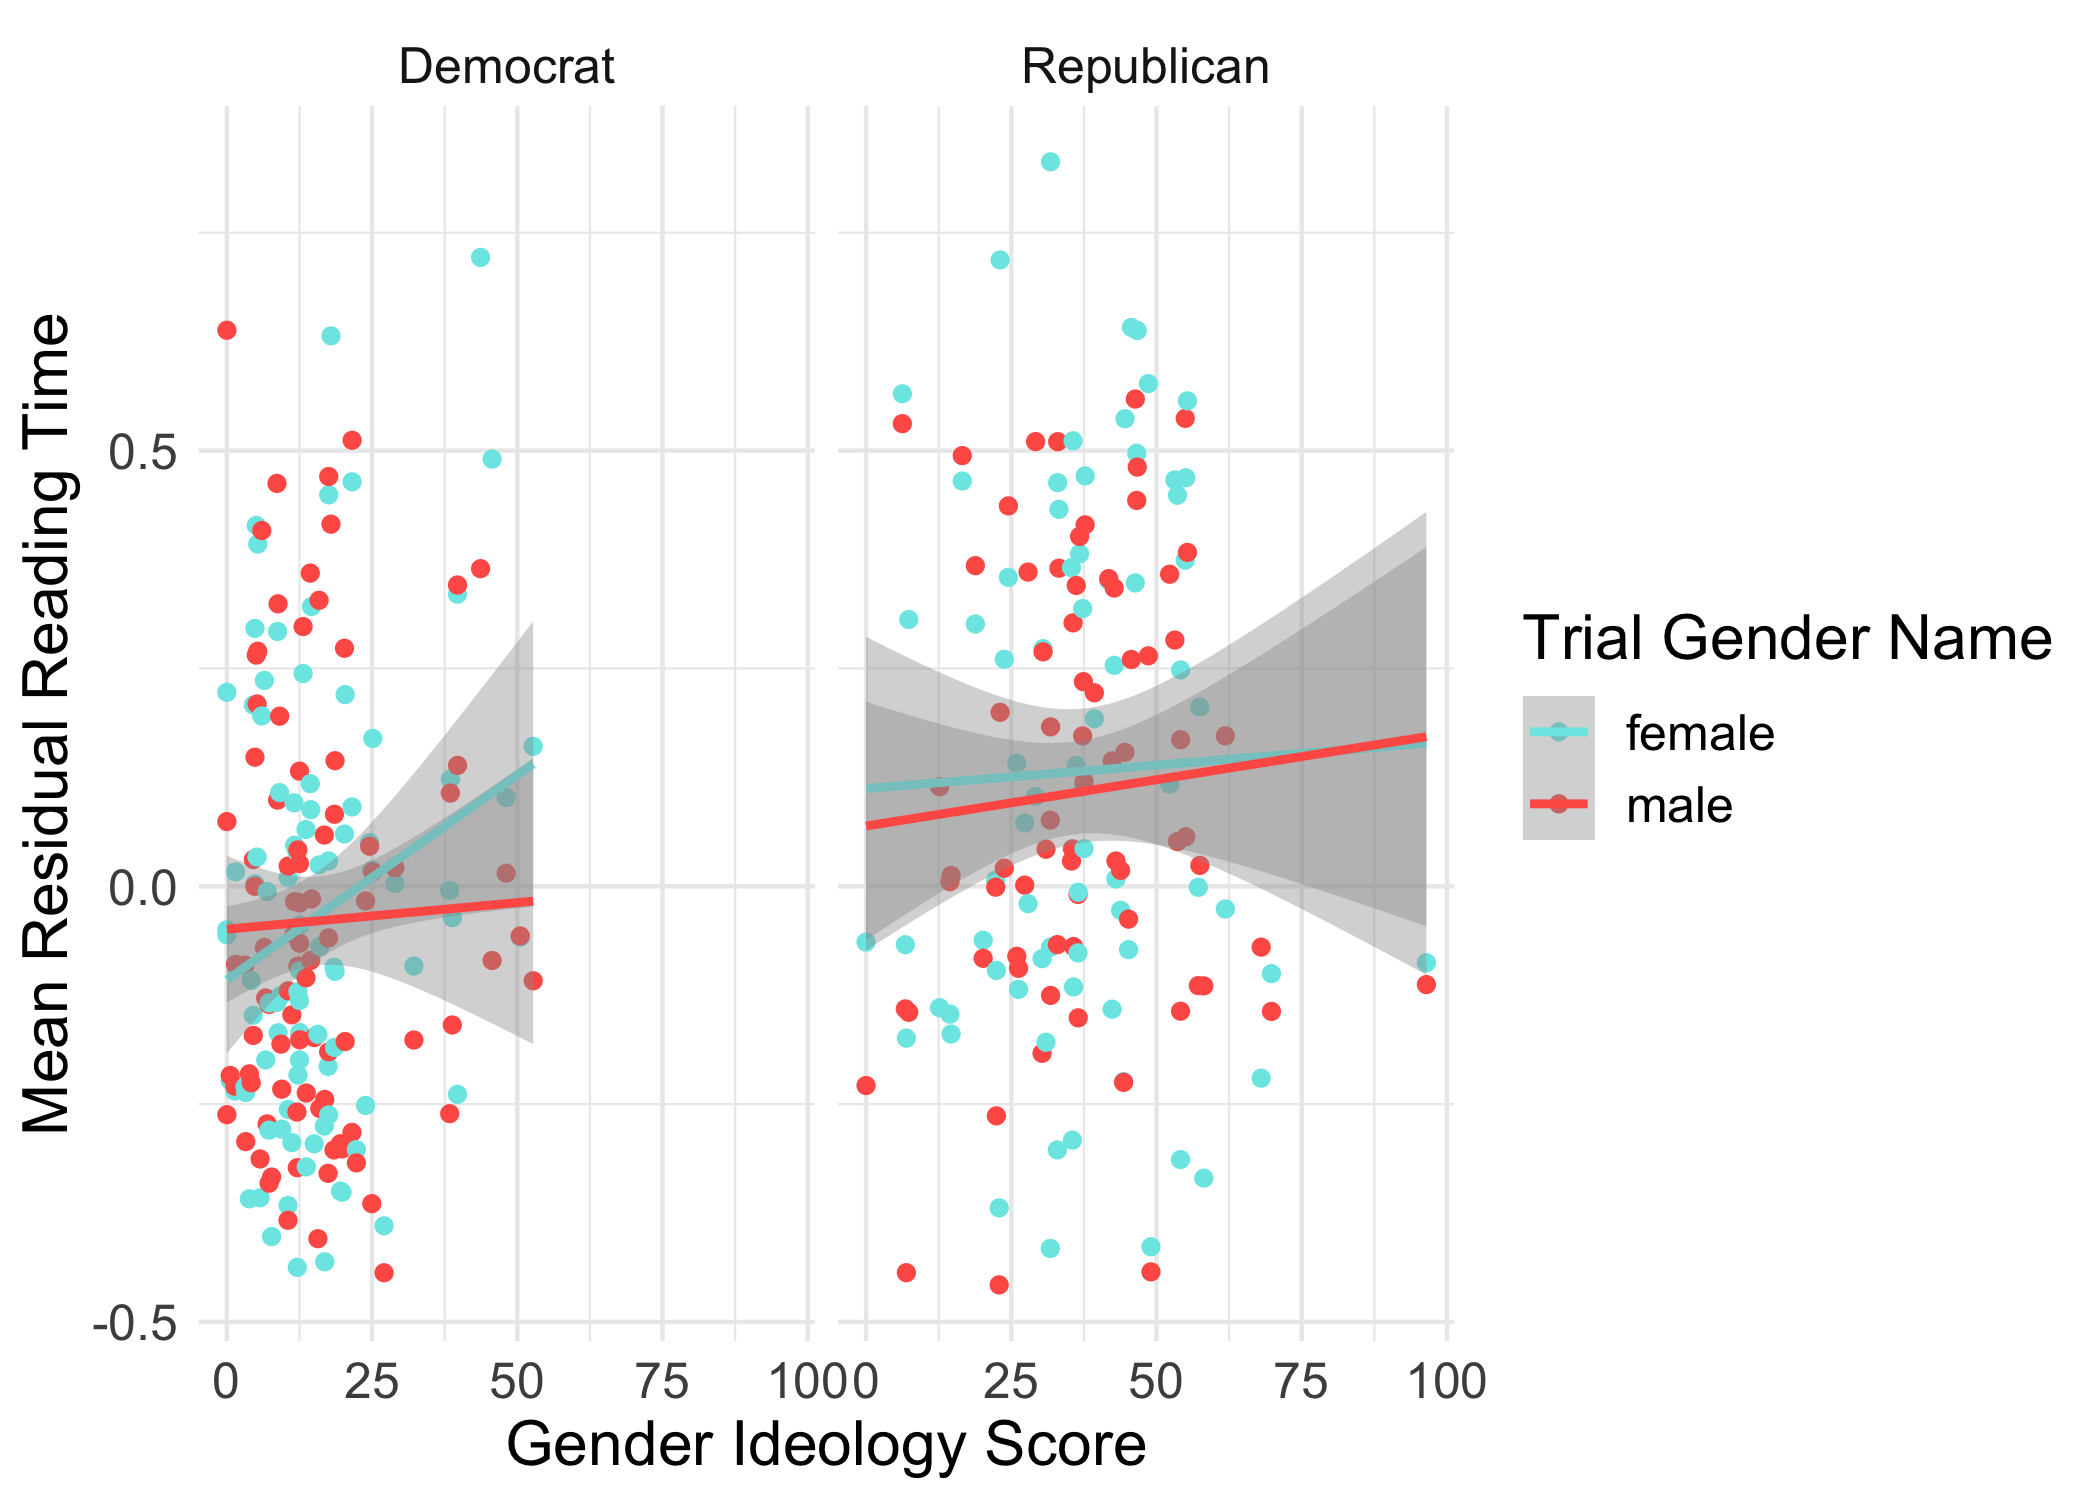
\includegraphics[scale=0.115]{maze_neutral_poli.png}
	%		\caption{Average residual decision time on gender-neutral forms in Experiment 1, faceted by political alignment.}
	%		\label{maze_neutral_poli}
	%	\end{figure}
%	
%	\newpage
%	\section{Experiment 2: Self-Paced Reading Task}
%	
%	\subsection{Methods}
%	
%	\subsection{Results}

Linguists have long been aware that individuals' and groups' orientations towards and away from particular identities, ideologies, or social groups influence the ways in which they engage with and employ their linguistic systems. This line of thinking can be traced back over 50 years, to Labov's seminal 1963 paper, which found that the residents of Martha's Vineyard produced diphthongs whose realizations were modulated by (or indexical of) their relationships to the island and its changing economic and cultural realities. More contemporarily, \textcite{podesva2015country} asserts that individuals from Redding participate in the California Vowel Shift to varying degrees, which are themselves a function of their orientation towards `town' (urban) or `country' (rural) identities. \par 
Beyond highly local identities, though not entirely removed from them, recent scholarship has linked the belonging of individuals to supralocal political groups as a predictor of linguistic production and perception. \textcite{hall2010indexing} found that Republicans in the United States House of Representatives were more likely to produce /\ae/ in the second syllable of \textit{Iraq} than their Democratic counterparts, who were more likely to produce /a:/. On the other hand, however, \textcite{hall2020breksit} find no such correlation in the production or perception of the voicing of the word-medial consonant cluster in the portmanteau \textit{Brexit}. Rather, the voiced variant /gz/ appears to index `whoever I think is wrong', regardless of what political belief the individual in question. So while not a predictor of linguistic production itself, the \textit{perception} of the cluster in \textit{Brexit} appears to be driven by political and personal ideologies.\par 
On the experimental front, there is a burgeoning landscape of literature investigating the relationship between ideology and personal beliefs as they relate to the processing and production of gendered language, which builds on previous work examining the relationship between societal expectations and reading times on gender-anomalous coreferents, such as \textit{he} for \textit{flight attendant} or \textit{she} for \textit{electrician} \parencite{foertsch1997search,duffy2004violating}. \textcite{von2020implicit} found that, in the context of the United States 2016 presidential election, participants' beliefs on whether or not Hillary Clinton would win the presidency had no effect on the production of \textit{she} as a coreferent pronoun with `the future president', and that `she' induced a processing penalty when read in a context in which it was coreferent with `the future president'. They did find that, in the context of the 2017 British General Election, coreferential \textit{she} was produced more frequently than \textit{he} when coreferential with the future Prime Minister, but that there was no such processing bonus for \textit{she} over \textit{he}, indicating lingering sexist beliefs in the realm of language processing, even when the incumbent (Theresa May) was female. Similarly, \textcite{pozniak2021failures} found that respondents who believed that female candidates would win in the 2020 Parisian and Marseille municipal elections were more likely to produce feminine-marked coreferential terms (both nouns and pronouns), but that masculine-marked forms were still dominant in both locales. \par 
While these studies present valuable insights into the ways in which individuals' beliefs about gender and specific referents influence their productions of gendered co-referents, they are limited in their generalizability in that they pick out real-world referents and events. Moreover, the diagnostic used to characterize individuals' beliefs specifically targets their predictions about real-world events, rather than their general ideologies towards gender. In order to investigate the question of how individuals' ideologies towards social categories such as gender may impact the production of gendered language, we conduct a forced-choice production task in which participants are tasked with assigning coreferential role nouns \parencite{misersky2014norms} marked for morphological gender to gendered characters in short fill-in-the-blank tasks. Such terms are one of only a small number of corners of the English language in which gender is still marked, by way of compounding (e.g. \textit{congress-man}, \textit{congress-woman}, \textit{congress-person}), though this is typically described as a manifestation of lexical, rather than grammatical, gender \parencite{kastovsky2011inflectional,hellinger2001english}. We examine these productions as a function of social ideology according to \textcite{baber2006social}'s Social Roles Questionnaire, and also as a function of political alignment. \par

\section{Experiment}

\subsection{Methods}
\subsubsection{Participants} 301 participants were recruited using Prolific. 100 Democrats and 100 Republicans were recruited initially, in order to maintain a political balance. All participants additionally self-identified as L1 English speakers and as having been born and in the United States, and all lived in the United States at the time of participation. None of the participants had participated in the pilot study or in any other study related to the present project. An additional 100 male-identifying participants were subsequently recruited do to a significant gender imbalance in the initial participant population (13.4\% male-identifying participants in the original population), as a result of an influx of female participants after Prolific went viral on social media app TikTok \parencite{charalambides2021}. The final gender-political distribution (after exclusions, see below) is provided in Table 1.\par
Participants were paid at a rate of \$15-\$16 an hour for their participation in the study, regardless of whether or not their data was used in the final analysis.

\begin{table}[!ht]
	\begin{center} 
		\caption{Participants by Gender and Political Orientation} 
		\label{sample-table} 
		\vskip 0.12in
		\begin{tabular}{llll} 
			\hline
			&  Democrat & Republican & Centrist\tablefootnote{These participants were recruited as either Democrats or Republicans, but reported a centrist identity in the post-experimental questionnaire} \\
			\hline
			Female &  82 & 62 & 25 \\
			Male & 42 & 46 & 10 \\
			Other & 4 & 0 & 0 \\
			Decline to state & 1 & 0 & 1 \\
			\hline
		\end{tabular} 
	\end{center} 
\end{table}

\subsubsection{Stimuli \& Procedure} All items in the experiment consisted of a complete sentence missing a single word. Participants were then provided with either two or three words which could complete the sentence by filling in the blank, and were asked to select the word which best did that. There were a total of 80 trials, with 20 critical items and 60 filler items.\par 
Critical items took the form ``[NAME] is a [blank] from [STATE]", where the blank was one of 14 social roles which shows a ternary distinction in its gender marking (e.g. \textit{congressman}, \textit{congresswoman}, \textit{congressperson}). An additional six critical items making only a binary distinction (e.g. \textit{villain} vs. \textit{villainess}) were also tested, but the results of these items are not reported on here. The twenty most popular male and female names were selected from the lists of most popular names for boys and girls in 1998 according to the Social Security \textcite{socialsecurity}. Names which appeared within the top 100 entries on both lists (e.g. Taylor, Ryan) were excluded, in order to ensure that the names used in the experiment were sufficiently socially gendered along binary lines. These names were randomized between participants, with no participant seeing the same name more than once. States and activities were randomized at the stimuli creation stage so that they remained constant for all participants.\par 
Filler items took one of two forms; semantic fillers and grammatical fillers. Semantic fillers had no prescriptively correct answer, and employed items from the same semantic field (1) or made use of common idioms or sayings (2). Some of these questions also dealt specifically with social and occupational titles and adopted the same syntactic frame as the critical items, in order to distract from the salience of gender in the critical items (3). 

\begin{exe}
	\ex That's the cutest (horse/Lusitano/equine) I have ever seen!
	\ex The (customer/parent/child) is always right.
	\ex Revati is a (writer/journalist/author) from India.
\end{exe}

Grammatical fillers, on the other hand, had prescriptively correct answers, and employed grammatical processes such as demonstrative selection (3), verb agreement (4), or preposition selection (5), among others. These items served a secondary purpose as attention check questions, and participants who answered incorrectly on more than 20\% of these questions were excluded from analysis (25 participants; see below).

\begin{exe}
	\ex She is typing on (\textbf{the}/these/those) computer.
	\ex Katherine (\textbf{sang}/song/sing) that song beautifully. 
	\ex They are they eating their soup (between/\textbf{with}/at) a spoon.
\end{exe}

All response possibilities, regardless of type (filler or critical) were shuffled between participants to control for possible ordering effects of presented options. As such, the examples in (1)-(6) are not necessarily indicative of the orders in which options were presented to participants. Similarly, all 70 trials were randomized between participants, after which they moved to the post-experimental phase of the study. 

\subsubsection{Post-Experimental Survey} In order to assess the participants' ideologies towards gender, we employ the Social Roles Questionnaire developed by \textcite{baber2006social}. This survey consists of 13 questions which are designed to elicit both implicit and explicit ideologies about gender, including the notions of gender as an immutable fact vs gender as a social construct (what Baber and Tucker term `gender transendence'), as well as about the societal roles performed by the (binary) genders (`gender linking').\par 
Each of the 13 questionnaire items was presented alongside a sliding scale from `strongly disagree' to `strongly agree', which corresponded to numerical values of 0 and 100, respectively. The questions related to `gender linking' were inversely coded. Participants were then assigned a gender ideology score from 0 to 100 by taking the mean of their individual responses; the closer to 0 a participant is, the more open-minded their approach to gender, and the closer to 100, the more conservative or traditional their view of gender.\par 
Finally, participants filled out an optional post-experimental demographic survey. This included questions about their own gender, political affiliations, and age. The full survey is available online as part of the supplementary materials.

\subsection{Results}
\subsubsection{Exclusions} 25 participants were excluded for not meeting the 80\% threshold for accuracy on the attention check questions. This yielded a total of 5,480 observations included in the final analysis.

\subsubsection{Response Gender by Political Party}
Responses were coded according to the gender which was seen in the target sentence; male names were coded as `male' stimuli gender and female names as `female' stimuli gender. We found that participants who identified as Democrats produced higher proportions of gender-neutral role titles than Republicans in both the male ($\beta$=-0.128, \textit{SE}=0.023, \textit{t}=-5.547, \textit{p}$<$0.0001) and female ($\beta$=-0.098, \textit{SE}=0.023, \textit{t}=-4.222, \textit{p}$<$0.0001) stimuli gender conditions, as highlighted in Figure 1.

\begin{figure}[ht!]
	\centering
	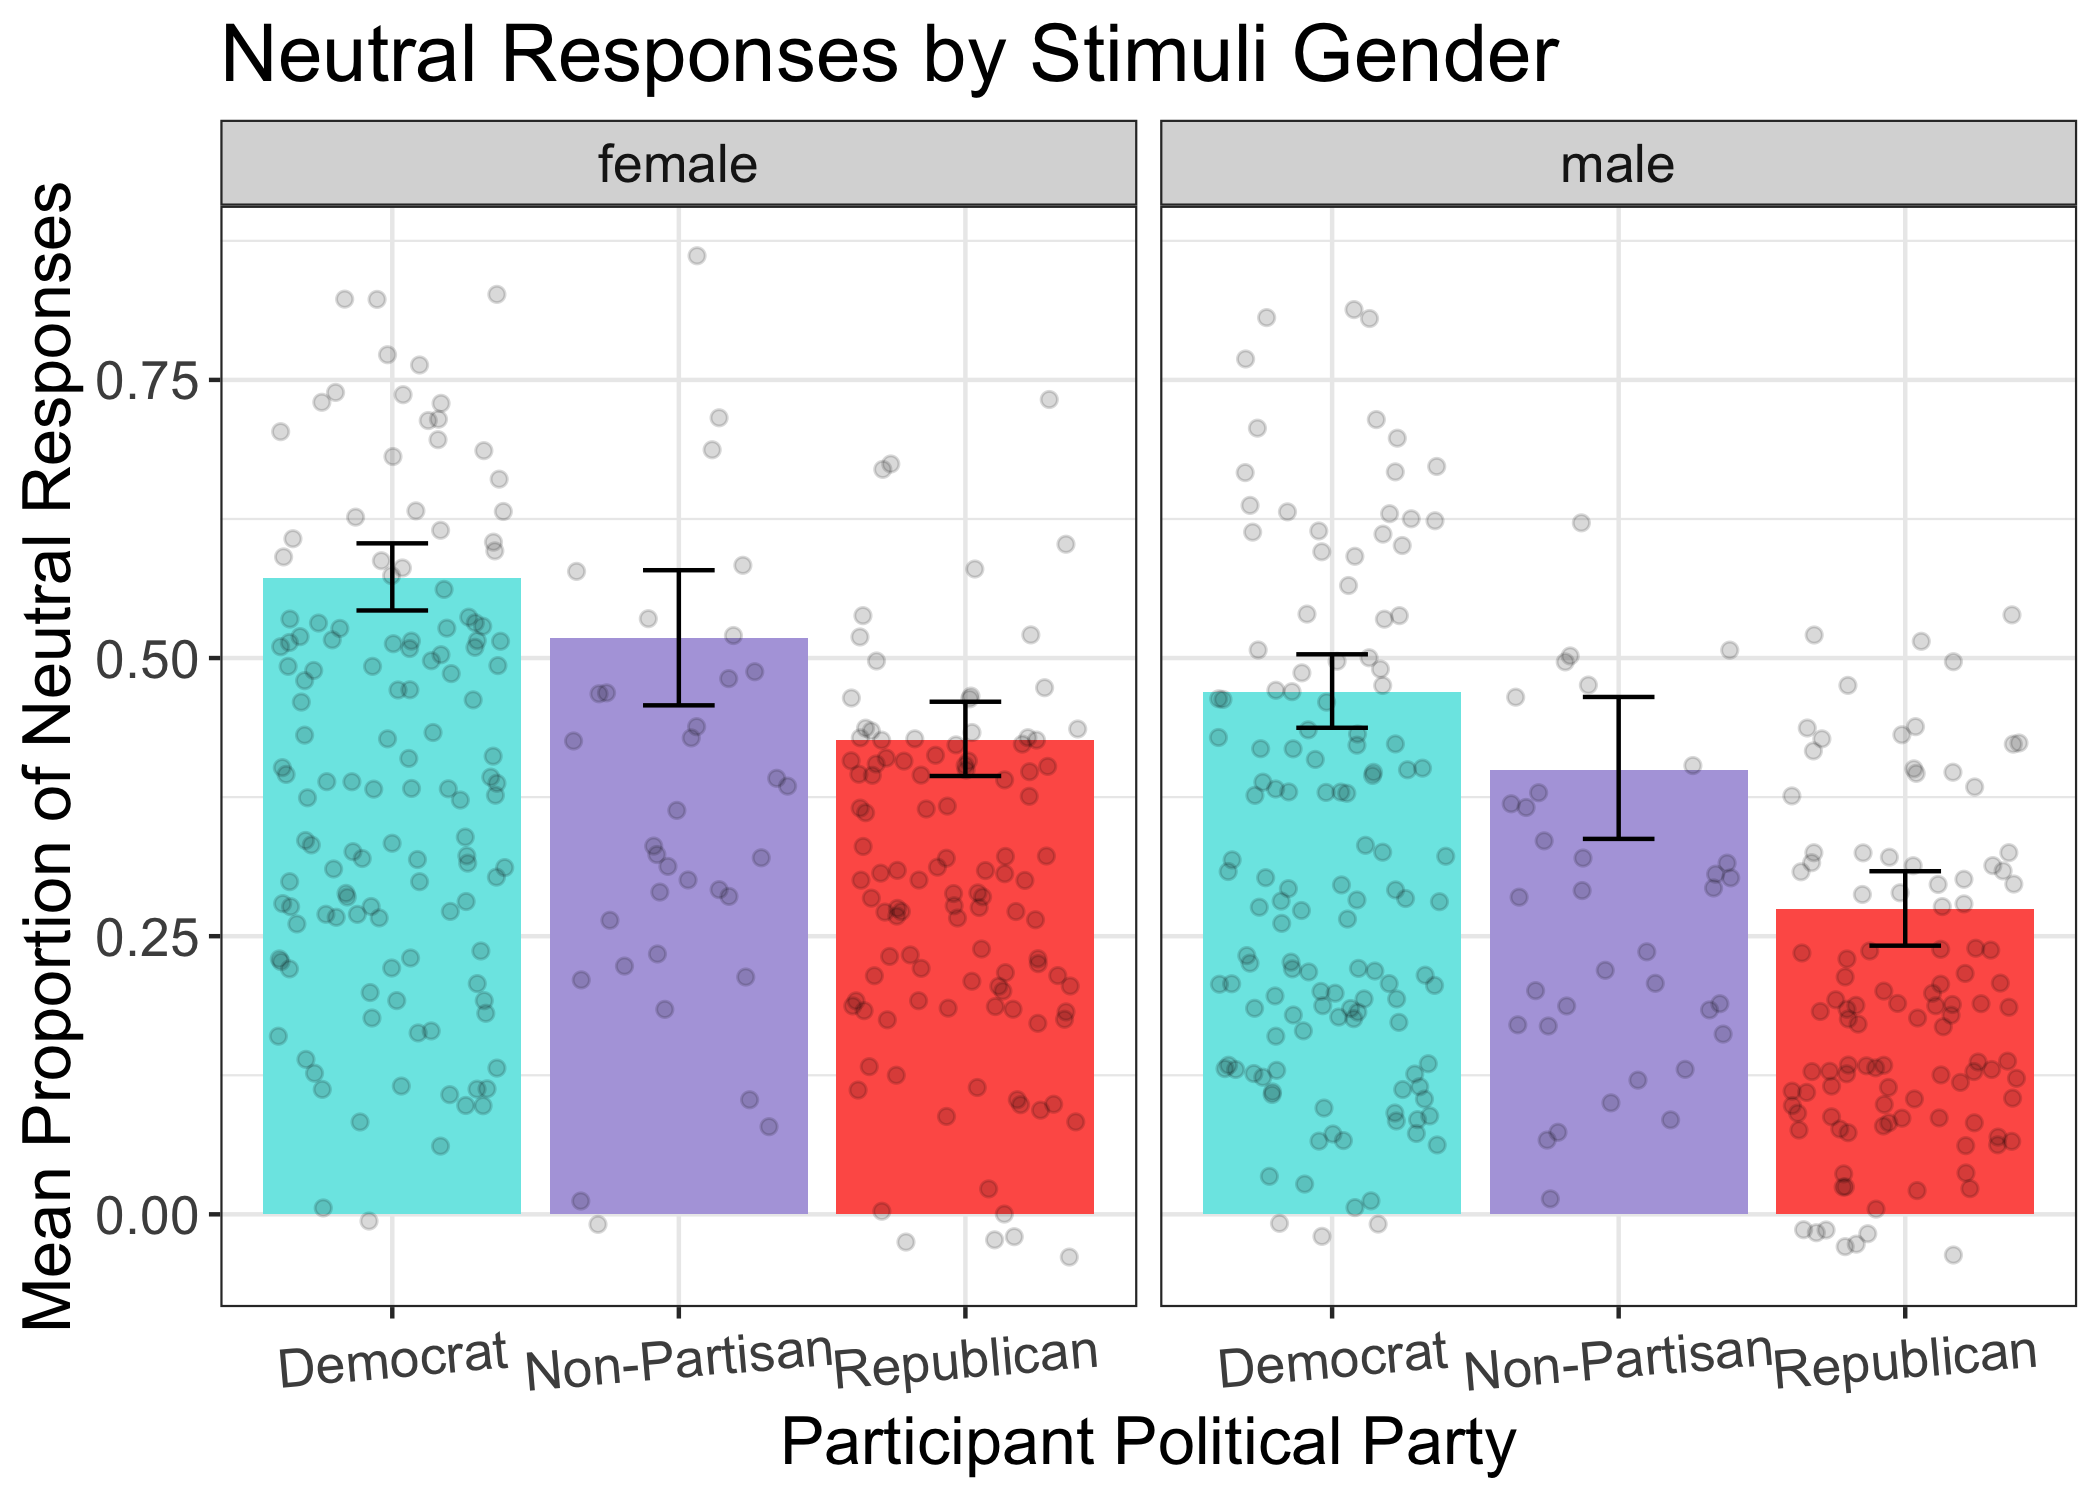
\includegraphics[scale=0.115]{prod_neutral_poli_bar_nonmean.png}
	\caption{Proportion of response genders by political party, faceted by gender of name in vignette seen.}
	\label{prod-box}
\end{figure}

Figure 2 shows the second principal finding of the role of stimuli gender; we observe that participants, regardless of political party, had higher rates of gender-neutral coreferential title productions when those titles were coreferential with female names than with male names  ($\beta$=-0.077, \textit{SE}=0.018, \textit{t}=-4.408, \textit{p}$<$0.0001). 

\begin{figure}[ht!]
	\centering
	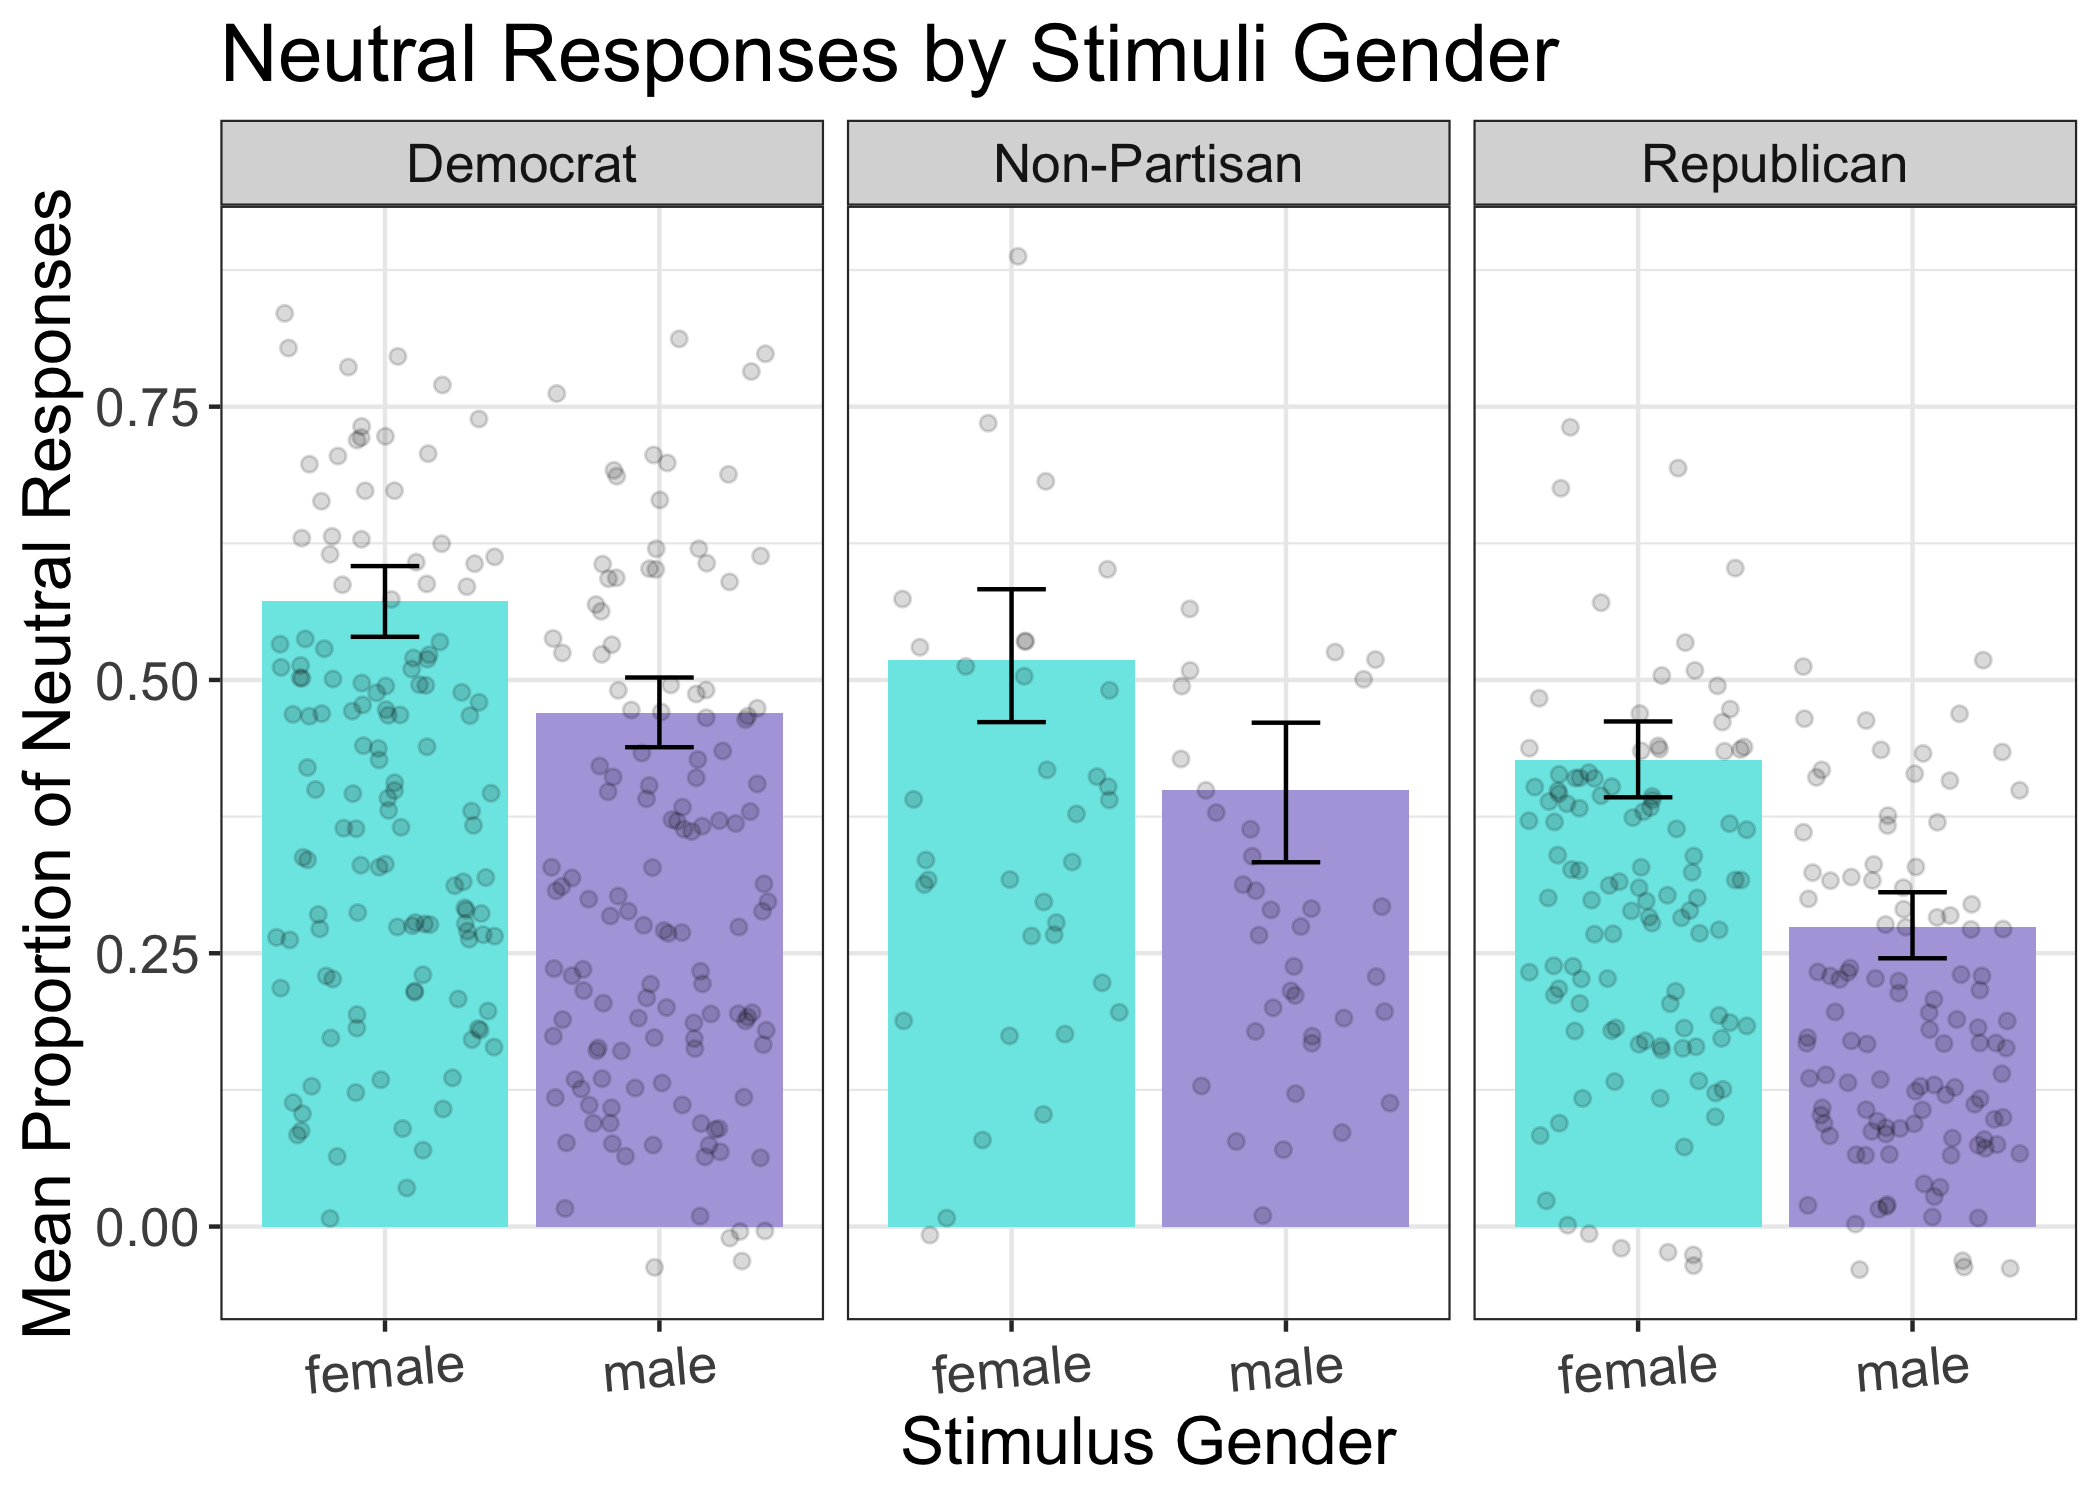
\includegraphics[scale=0.115]{prod_neutral_gender_bar_nonmean.png}
	\caption{Average proportion of neutral responses as a function of gender ideology, faceted by political alignment.}
	\label{prod-neutral-poli-box-gender}
\end{figure}

\subsubsection{Response Gender by Political Party \& Individual Ideology}
We turn now to the more fine-grained issue at hand, which is the role of individuals' ideologies about gender in their production of gender-neutral forms. Highlighted in Figure 3, we find that ideology does have a significant effect on the proportion of gender-neutral coreferential role titles produced, but that this is driven by Democrat-identifying participants ($\beta$=-.006, \textit{SE} = 0.001, \textit{t}=-5.345, \textit{p}$<$.0001), as Republican-identified participants show no such significant effect ($\beta$ = 0.000, \textit{SE}=0.000, \textit{t}=-0.382, \textit{p}$<$0.703). That is, Democrats with more conservative gender ideologies produce lower proportions of gender-neutral terms than Democrats with more progressive gender ideologies, while Republicans rates of gender-neutral productions stay relatively stable, regardless of the individual's ideology towards gender.

\begin{figure*}[ht!]
	\centering
	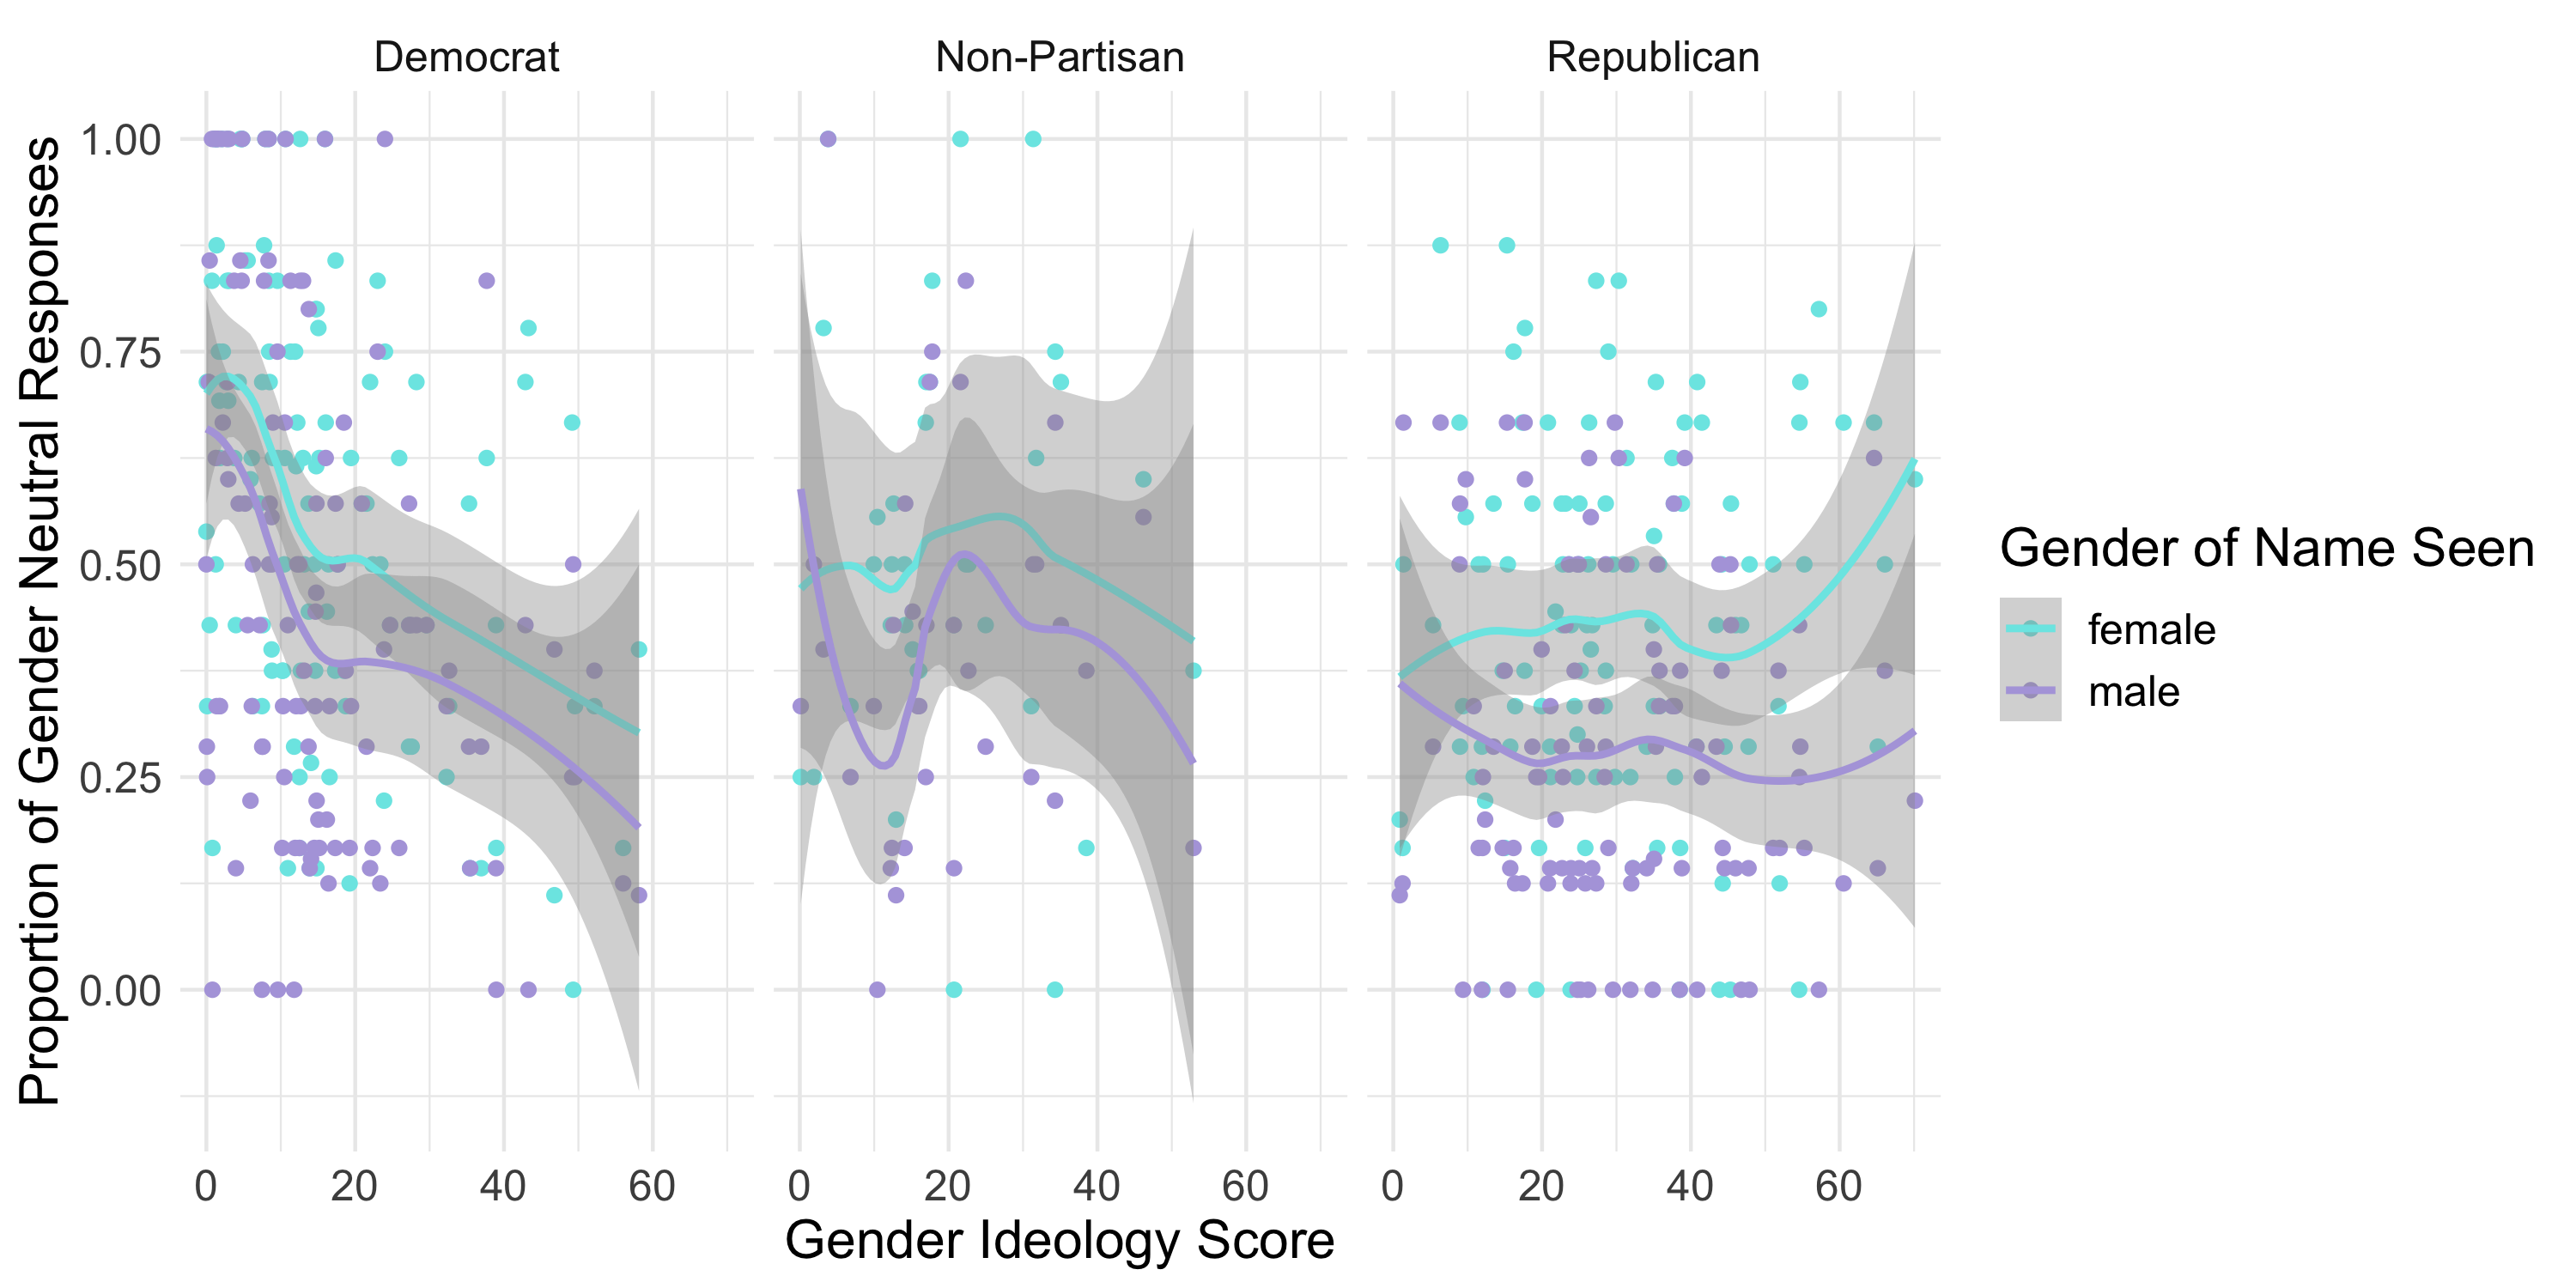
\includegraphics[scale=0.15]{prod_neutral_poli.png}
	\caption{Average proportion of neutral responses as a function of gender ideology, faceted by political alignment.}
	\label{prod-neutral-poli}
\end{figure*}
\section{General Discussion}

\subsection{The Female Effect in Gender Neutral Productions}
Of note in the findings is that female coreferential names are consistently more likely to be assigned gender-neutral role titles than their male counterparts. This is perhaps surprising, as, with the singular exception of \textit{flight attendant}, all of the neutral forms in our norming study were evaluated as either equally likely to be of either gender, or significantly more likely to be describing a male referent\footnote{The full results of the norming study are available in the online supplementary materials}. These findings are presented in Figure 4.

\subsection{The Role of Political Ideology in Gender Neutral Productions}

\section{Acknowledgments}

\section{Supplementary Material}
Supplementary materials, including details related to the norming study and unreported processing studies, can be found at \url{https://branpap.com/qp1-supplementary-materials}.

\nocite{labov1963social}



	Participants were paid at a flat rate of \$1.75, with a mean completion time of 5.51 minutes (before exclusions). This resulted in an average rate of \$20.73/hr. Participants received payment regardless of their inclusion in the final analysis.
	
		Participants were paid at a rate of \$15-\$16 an hour for their participation in the study, regardless of whether or not their data was used in the final analysis.
	

Critical items took the form ``[NAME] is a [blank] from [STATE]", where the blank was one of 14 social roles which shows a ternary distinction in its gender marking (e.g. \textit{congressman}, \textit{congresswoman}, \textit{congressperson}). An additional six critical items making only a binary distinction (e.g. \textit{villain} vs. \textit{villainess}) were also tested. \par 

	\section{Supplementary Materials}
Supplementary materials, including details related to the norming study and the unreported processing study, can be found at \url{http://www.branpap.com/research.html}.

	Participants who failed to accurately respond to at least 85\% of the attention check questions were excluded from analysis. 19 participants were excluded on this basis, for a final total of 279 participants whose data were included in the analysis (6.3\% exclusion rate). \par 
	
25 participants' data were excluded for failing to reach the 80\% threshold on attention check questions, for a total of 276 participants whose data was analyzed (8.3\% exclusion rate).\par

This set of exclusions leaves us with a final set of 5179 analyzable observations.

Taken together with the results of \textcite{pozniak2021failures}, it appears that individual expectations about events or gender roles do indeed modulate the production of gendered language.

%	Finally, we observe in the processing task that the effect of frequency is markedly more predictive for the young participants than it is for the older participants. While not directly related to the question at hand, it bears mentioning here due to the politically charged nature of the data. One possible interpretation of this finding is that young people are not consuming the kinds of mainstream media that are reflected in COCA, and as such are not receiving the same kind of input on politically charged terms as their elders. If this is the case, it has larger-reaching implications for the ways in which we implement frequency estimations into our linguistic analyses, and we believe this discrepancy and the related line of inquiry deserve further investigation. \par 

The existence of overt commentary on the employment of gender-neutral role titles in the public sphere further substantiates this interpretation. 

and employed items from the same semantic field (7) or made use of common idioms or sayings (8). Some of these questions also dealt specifically with social and occupational titles and adopted the same syntactic frame as the critical items, in order to distract from the salience of gender in the critical items (9). 

 to control for possible ordering effects of presented options
 
 As such, the examples in (1)-(6) are not necessarily indicative of the orders in which options were presented to participants.
 
 The demographic breakdown of the participants whose data was included in Experiment One is provided in \hyperref[exp1-sample-table]{Table 1}
 
 None of the participants had participated in the pilot study or in any other study related to the present project.
 
 This resulted in the previous word disappearing and the subsequent one being revealed on the screen
 
 , since each of these questions had a vignette-internally correct answer
 
 The final gender-political distribution is provided in \hyperref[exp2-sample-table]{Table 2}
 
 While none of the participants in our norming study reported being unfamiliar with any of the female terms
 
 These opposite poles of the spectrum were termed `gender progressive' and `gender conservative', respectively.
 
 